
\chapter{Introduction}


    


Humans have a remarkable ability to perceive visual stimuli emanating from the world around them. Not only do we identify different objects, scene depth, movement, and colour with ease, but visual scenes might even elicit enjoyment and meaning in our lives. Man-made machines on the other hand are much more easily decomposed into a set of deterministic modules that require explicit, well defined instruction sets. This thesis is concerned with developing a set of algorithms that breaks down, and utilises the wealth of information in image data to produce valuable signals that can be employed in robotic perception. 


\section{Motivation}
\subsection{Visual Odometry and Robotic Perception}
True  autonomy in mobile robotics requires the ability to perceive the world adequately. In particular, understanding the structure and size of the space inhabited by the robot, as well as its own movement through that space are vital to its ability to navigate and interact with the world. Computer vision algorithms in combination with increasingly lower-cost and higher quality imaging hardware offers a popular solution, encompassing enormous diversity in sensing modalities and precipitating the development of powerful perception systems in modern robotics. Plenoptic imaging is one such expression of evolving imaging technologies that continues to yield promising results in tasks such as mapping \cite{kuehefuss2016rgbdslam}, underwater imaging \cite{skinner2016underwaterplenoptic}, low light imaging \cite{dansereau2015volumetric}, and classification \cite{wang2016lfcnn}.

This work is concerned with the application of \textbf{plenoptic imaging} in two intimately related tasks: \textbf{visual odometry} which involves estimating the motion of a camera in 3D space, and \textbf{depth reconstruction} which estimates the shape of the scene in an image. We elucidate the motivation for addressing these challenges by looking at one of the most important challenges currently being tackled in robotics: localisation and navigation. A robot's locale is a vital piece of information required to effectively plan paths and navigate through any environment. The challenge however, is that localisation typically requires a map of the space. In an unknown environment where a map doesn't exist, the robot must simultaneous tackle the problems of reconstructing the environment's geometry, and localising itself within that geometry. This is a challenge known as SLAM (Simultaneous Localisation and Mapping), and has proven a challenging robotics problem for at least 30 years \cite{cadena2016slam, kuehefuss2016rgbdslam}. Odometry is a crucial component of even the most sophisticated SLAM algorithms. In this work, odometry is treated as a problem which can be tackled with visual perception and computer vision algorithms. 

\begin{figure}[htbp]
    % \centering 
    \subfloat[Spot (Boston Dynamics)]{
        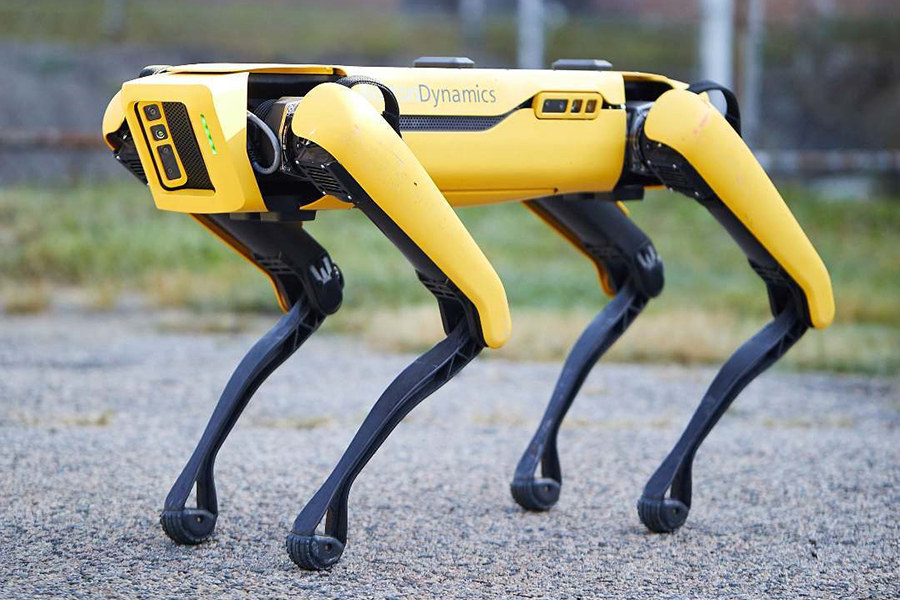
\includegraphics[height=1.33in]{images/spot.jpg}
    }
    \subfloat[AUV Sirius (ACFR)]{
        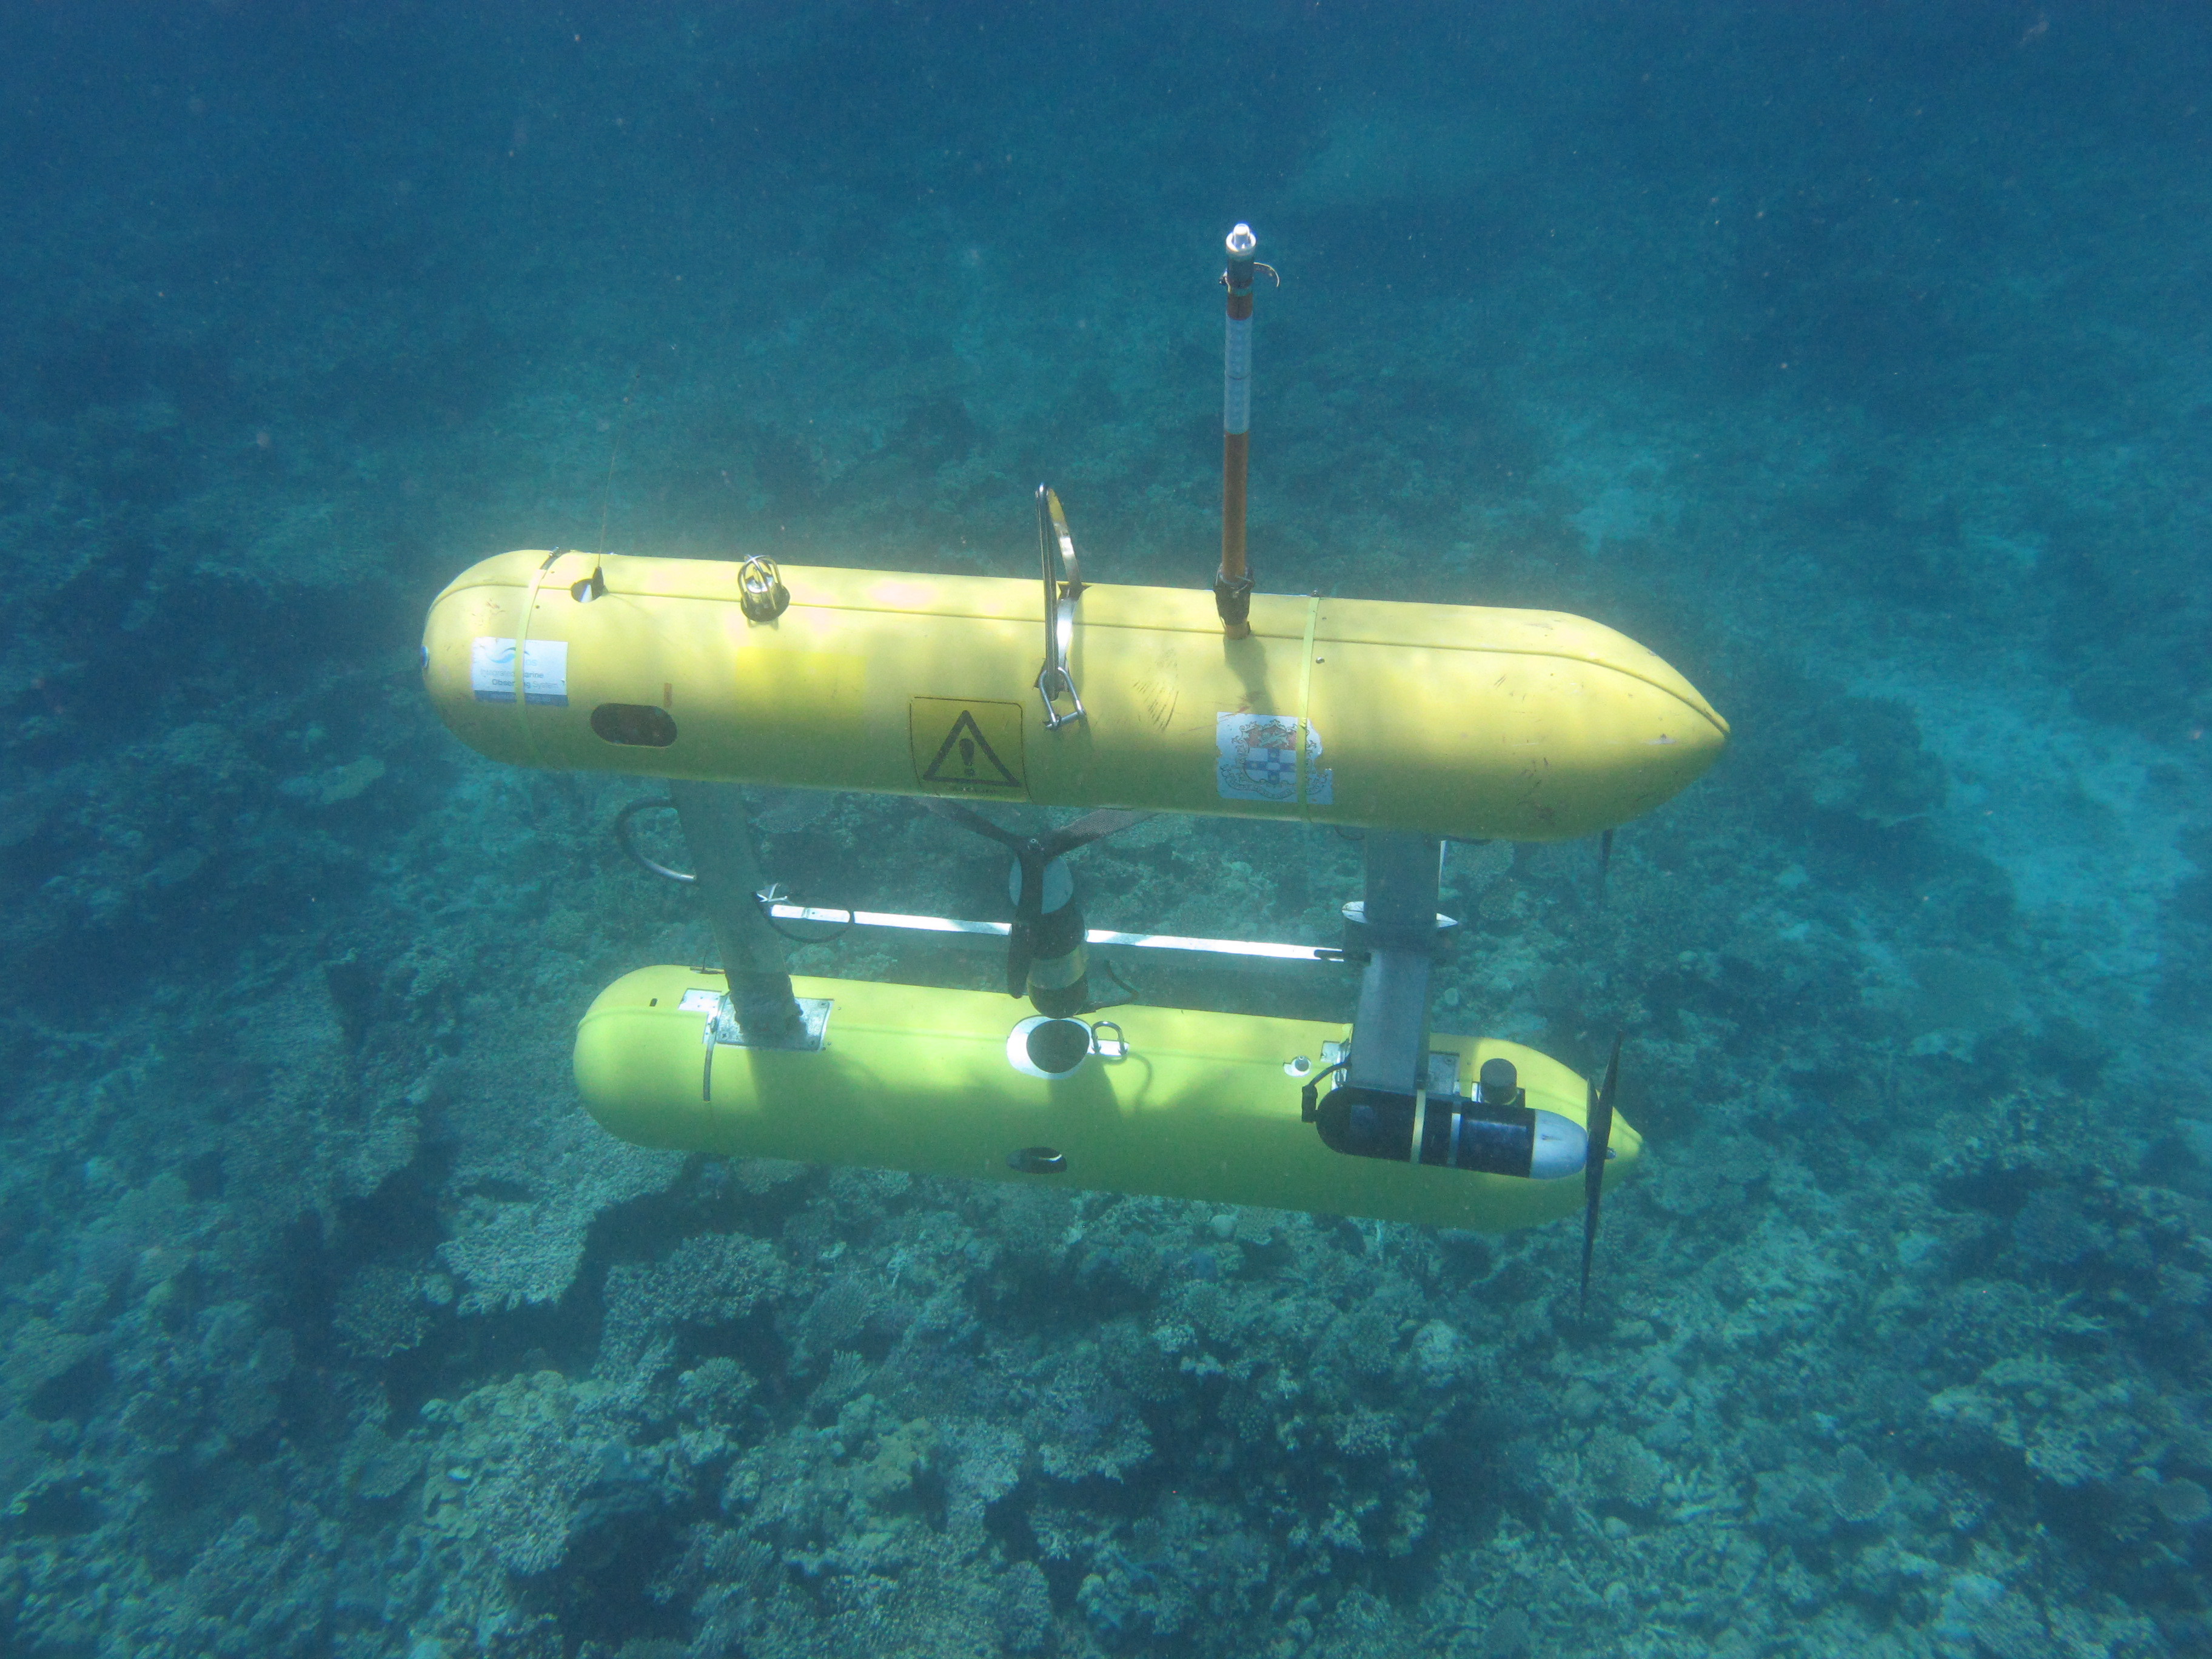
\includegraphics[height=1.33in]{images/rov_sirius.jpg}
    }
    \subfloat[Troika (LG)]{
        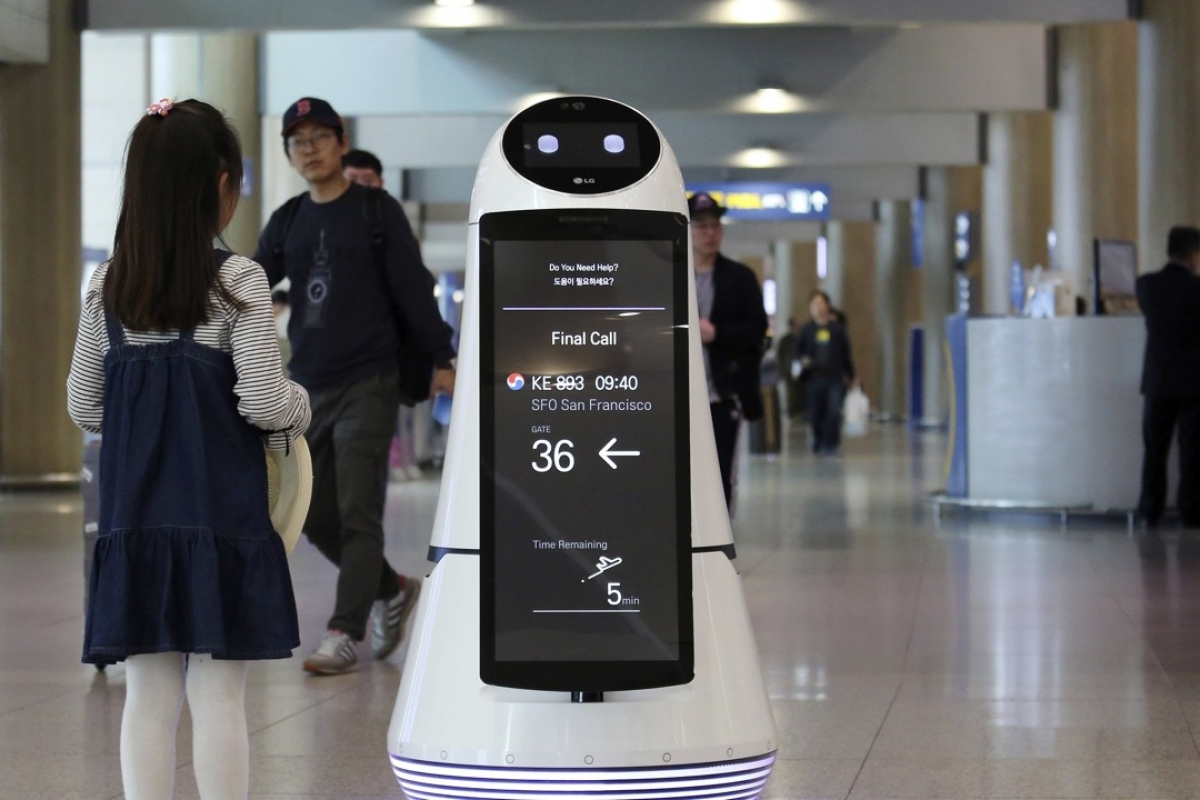
\includegraphics[height=1.33in]{images/troika.jpg}
    }
    
    
    \caption[Examples of robots that operate in unconstrained spaces.]{Autonomous mobile robots are increasingly operating in unconstrained environments, characterised by uneven terrain, weak GPS signal or crowds of moving people. An important challenge for the broader adoption of these types of mobile robots, is navigational capabilities, which rely foundationally on mapping and localisation algorithms.}
\end{figure}


One might question the practicality of using image data for these tasks when great success has been found with more specialised sensing modalities; motion estimation for example is typically addressed with inertial sensor measurements or Global Positioning System (GPS) receivers. Other robotic systems employ lidar, acoustic range-finding, time-of-flight cameras or structured-light cameras to gain access to 3D models of the environment. Cameras however, can often offer superior tradeoffs in size, weight, cost, power consumption, and they deliver a rich, highly detailed representation of the world. Furthermore, unlike \textit{active} sensor technologies which sense the world by `illuminating' it, cameras are \textit{passive} sensors, meaning they do not interfere with one another and can be employed in a more diverse range of environments. Thanks to their ability to adjust their exposure period, aperture size and sensor gain, cameras are also highly capable in a variety of lighting conditions and environments. 

Furthermore, the applications of visual odometry extend beyond the context of SLAM algorithms. For example, a multi-rotor Unmanned Aerial Vehicle (UAV) can fuse measurements from inertial and visual measurements to hover in place in GPS denied environments. Outside of the field of robotics, Augmented Reality (AR) applications are employing visual odometry and SLAM to render virtual 3D models in real time on top of camera feeds. Proença \cite{proenca2018rgbd} envisages an AR application that employs visual odometry to guide an operator through a contaminated nuclear facility, whilst rectifying existing 3D models of the facility. The adversities of installing guidance and navigation infrastructure in such facilities can be extrapolated to cases such as planetary rovers and Remotely Operated Underwater Vehicles (ROVs).


\subsection{Computational Imaging}

Visual perception is attractive for robotics for many reasons, however, as with any kind of system design, the tradeoffs need to be considered. Digital cameras accumulate photons at each pixel, forming an image after a brief period of `exposure' - the longer the exposure, the brighter the image. However, cameras that move - as robots often do - are likely to accumulate motion blur. Alternatively, a larger aperture accumulates a larger number of photons, but gives rise to shallow depth-of-field - an aesthetically pleasing effect in photography, but a limitation for computer vision algorithms. 

\textit{Computational photography} unifies the design of optics, algorithms, sensors and illumination to capture better photographs. Modern smartphones, as an example, have relatively slow lenses, small sensors, and cheap optics. DSLR and mirrorless cameras on the other hand take advantage of higher grade optics and larger sensors - which might lead us to expect better image quality compared to phone cameras. Modern smartphones however benefit from powerful CPUs, hardware-accelerated graphics, and an entire community of software engineers working on algorithms. Many of the effects that were once unique to expensive imaging devices can now be replicated on smartphones. Low light imaging is enhanced using algorithms such as Google's `Night Sight' \cite{levoy2019lowlight} to improve clarity and colour accuracy. Shallow depth-of-field, an effect that is typically difficult to capture on a wide lens with narrow apertures is now replicated using `Portrait Mode' \cite{wadhwa2018portraitmode}.

In this work, we embrace computational imaging as a modern approach to visual odometry. Humans are exceptionally well adapted to tasks involving visual motion and depth perception - our two eyes let us process the 3D geometry of a scene, while our learned experiences are often able to fill in the gaps where geometric information is insufficient or unavailable. Image processing algorithms are not equipped with this same kind of human intuition, and so the deceptively complex task of estimating the 3D structure of a scene from a sequence of images continues to attract attention from the computer vision community \cite{dansereau2011plenopticflow,gakne2018scale,nister2004vo,zhou2019scale}. 

The price of camera components is decreasing while image quality continues to improve, not only making cameras an attractive perception module for autonomous robotics, but also spurring the popularity of multiple-view imaging. Embracing this idea, this work adopts vocabulary from the literature on light field imaging, applying this promising imaging technology to the tasks of visual odometry and depth perception. More broadly however, the principle underpinning much of this thesis is that novel imaging devices that break away from the traditional pinhole model of the camera have vast implications in the field of machine vision. We need not look any further than the animal kingdom to see why this is true - the biological eye is estimated to have evolved independently no fewer than 50 times, each variant acutely adapted to the particular set of challenges in their environment. The diversity and evolutionary ingenuity in biological visual perception systems prompts an important question in robotics and computer vision - how best should we equip robots to see the world given a particular set of challenges and environments? In this thesis, a camera array which is a simple yet versatile extension of the stereo camera is used to develop the algorithms that address the visual odometry and depth reconstruction problems. 



\section{Problem Statement}

There is a well established library of solutions addressing the visual odometry and depth reconstruction problems. Some use closed form solutions that directly solve for geometry and ego-motion, while others, like this work utilise a data-driven approach to indirectly model visual odometry. Throughout this work, we will refer to these as the \textit{geometric} and \textit{data-driven} approaches, both of which form a crucial part of our survey of existing state-of-the-art methods

This thesis tackles the problem of estimating visual odometry and depth using an \textit{uncalibrated} camera array - a challenge that, to the best of our knowledge, is absent in existing state-of-the-art methods. Robots operating in unconstrained environments are typically exposed to destabilising effects including thermal expansion, vibration and shock - effects which might render the calibrations of camera arrays invalid. Multiple-view geometry, which is harnessed by the \textit{geometric} family of algorithms, is materially dependent on knowing the orientation and position of the cameras; rotating a camera even a few arc-seconds from its calibrated position results in a disproportionally magnified error in the image being formed. 

Existing \textit{data-driven} approaches on the other hand, have typically used monocular or stereo imagery, overlooking the richness of light field imagery as a possibility for improving robustness and accuracy. Within the data-driven family of algorithms, a relatively new \textit{unsupervised} approach has emerged, cleverly piecing together the available information to learn visual odometry from raw footage alone. The unsupervised nature of this approach means that the model calibrates itself in a fashion, learning from raw data to produce ego-motion predictions. Unsupervised machine learning makes `online-learning' possible, in which models take advantage of new data becoming available in-situ, improving performance and building robustness to different environments. Most importantly however, unsupervised models are able to adapt to errors in the calibration of the equipment without requiring hand-labelled data to supervise the learning process. A self-calibrating and adaptive perception module which is robust to adverse effects is an attractive capability in robotics. Once again however, existing unsupervised algorithms have not been applied to light field data, prompting a natural, yet important next step which is the subject of this work: combining the richness of light field data with the self-calibrating capabilities of unsupervised learning algorithms to perform visual odometry.



\section{Contributions}
This work builds on existing data-driven approaches, suggesting an adaptation of conventional 2D machine learning algorithms to enable unsupervised learning on light field data. Specifically, we make the following contributions: 

\begin{itemize}
    \item We adapt 2D unsupervised algorithms for learning depth and pose, suggesting a generalisation of existing algorithms that enables them to operate on arrays of cameras.
    \item Through this adaptation, we show that our approach is not only scale-consistent, but also grounded in metric depth and pose measurements. 
    \item We suggest three encodings of the light field which are well suited to 2D convolutions, making them convenient for ingestion using convolutional neural networks. 
    \item We demonstrate that our algorithm outperforms existing state-of-the-art approaches using monocular imagery, reinforcing the benefits of light field technology in robotic imaging. 

\end{itemize}


\section{Outline}
Concepts from computer vision, machine learning and light field imaging are used heavily throughout this thesis, and \textbf{Chapter 2} begins by providing an overview of the relevant background information. On the subject of computer vision, it describes the pinhole model of the camera, the fundamentals of multiple view geometry, and develops intuition relevant to light field imaging. Machine learning is presented as an approach to solving computer vision problems, with emphasis directed towards convolutional neural networks, as an algorithm that continues to gain popularity in image based problems.

The existing approaches for performing visual odometry and depth estimation are reviewed in \textbf{Chapter 3}, presented in two categories: geometric approaches which rely on directly modeling movement through 3D space, and machine learning approaches which take advantage of massive datasets to build resilient, data-driven solutions.

\textbf{Chapter 4} introduces a novel light-field based algorithm for simultaneously learning depth and pose. We begin by describing a simple extension of existing monocular approaches, then proceed to layer-in modifications that enforce scale-consistency, and metric pose estimates, taking advantage of 4D light field data. We also describe our experimental setup, including our data acquisition strategy using a robotic manipulator to collect a suitable 4D video dataset. 

In \textbf{Chapter 5} we presents results from our two proposed algorithmic pipelines, and compare these to state-of-the-art existing methods. We demonstrate that our approach outperforms monocular approaches in both depth and pose estimation. Furthermore, we show results for our experiments with three light field encodings, with the intention of empirically comparing the effectiveness of different input methods.

An in-depth discussion on the successes and challenges in this work is provided in \textbf{Chapter 6}, with specific detail on the effectiveness of our two pipelines and three input methods. 

Finally, we conclude this work in \textbf{Chapter 7}, drawing conclusions from our experimental results on the promise of light field and deep learning technologies, and suggest some potential applications and future research questions to continue the spirit of our work. 
